\chapter{ Экспериментальный раздел}

В данном разделе будут произведены замеры времени работы алгоритма. Для исследования скоростных характеристик был использован компьютер на базе процессора Intel Core Intel(R) Core(TM) i5-8250U CPU @ 1.60GHz, содержащий 8 Гб оперативной памяти.

\section{ Тестирование алгоритма}

Для проверки значимости Q -- параметра, имеющий значение порядка длины оптимального пути, зафиксируем значения $\alpha$ $\beta$ и p и будем изменять Q  в диапазоне [0, 50] с шагом 1. Результаты приведены на \ref{fig:timefor_q}

\begin{figure}[ht!]
    \centering{
        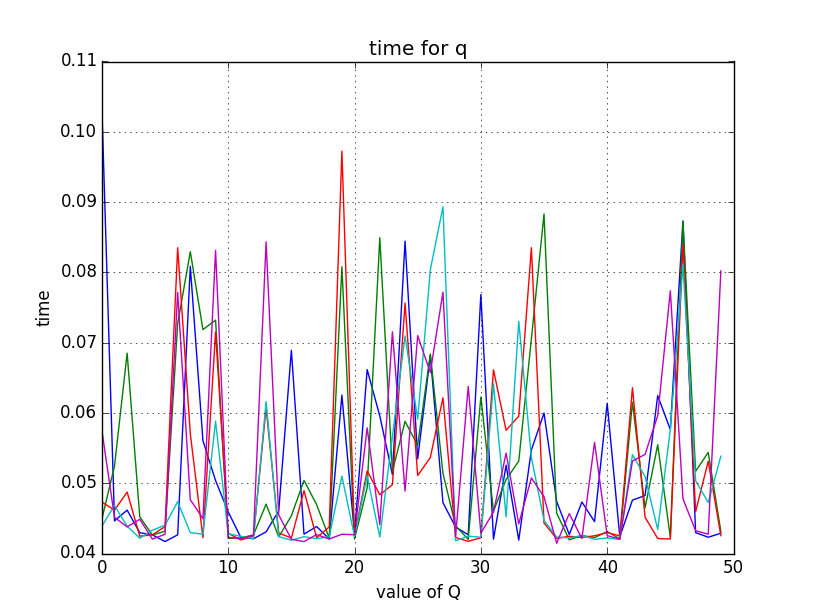
\includegraphics[width=1.1\textwidth]{img/timefor_q.png}
    \caption{ График, отображающий зависимость времени работы алгоритма от параметра Q}
    \label{fig:timefor_q}
    }
\end{figure}

Для проверки значимости параметра $\alpha$, зафиксируем Q=1, $\beta$=0 и p=0.5 и будем изменять $\alpha$ в диапазоне [0, 5] c шагом 0.5. Результаты приведены на \ref{fig:timefor_alpha}

\begin{figure}[ht!]
    \centering{
        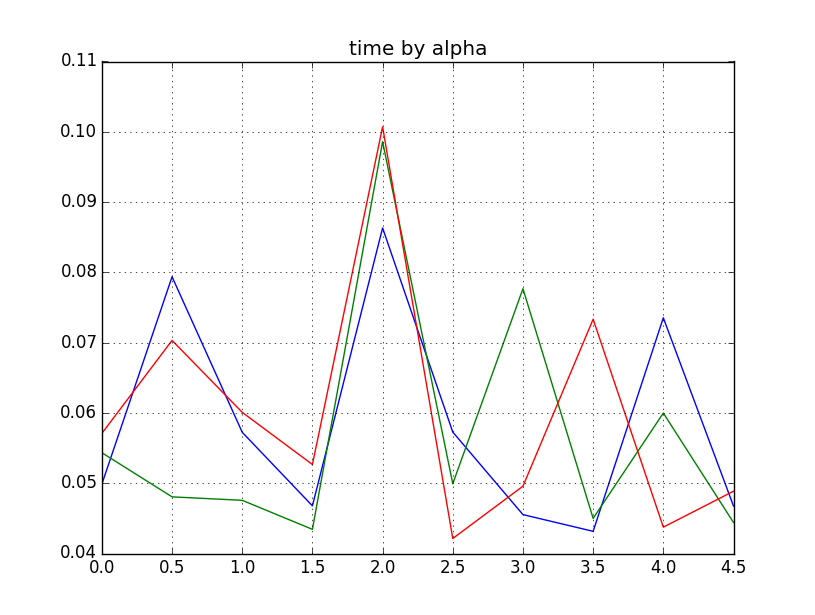
\includegraphics[width=1.1\textwidth]{img/timefor_alpha.png}
    \caption{ График, отображающий зависимость времени работы алгоритма от параметра $\alpha$ }
    \label{fig:timefor_alpha}
    }
\end{figure}

Для проверки значимости $\beta$, зафиксируем Q=1, $\alpha$=0 и p=0.5 и будем изменять $\beta$ в диапазоне [0, 5] с шагом 0.5. Результаты приведены на \ref{fig:timefor_beta}

\begin{figure}[ht!]
    \centering{
        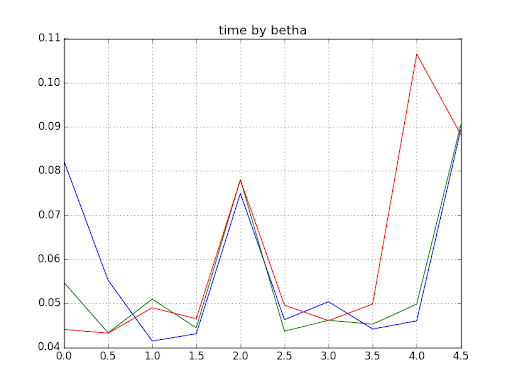
\includegraphics[width=1.1\textwidth]{img/timefor_beta.png}
    \caption{ График, отображающий зависимость времени работы алгоритма от параметра $\beta$ }
    \label{fig:timefor_beta}
    }
\end{figure}

Как видно из \ref{fig:timefor_alpha} и \ref{fig:timefor_beta} у параметров $\alpha$ и $\beta$ есть "нежелательное" значение, равное двум, на котором алгоритм работает неэффективно.

Для проверки значимости e, зафиксируем Q=1, $\alpha=1$, $\beta$=1 и p=0.5 и будем изменять e в диапазоне [0, 5] с шагом 0.5. Результаты представлены на \ref{fig:timefor_e}

\begin{figure}[ht!]
    \centering{
        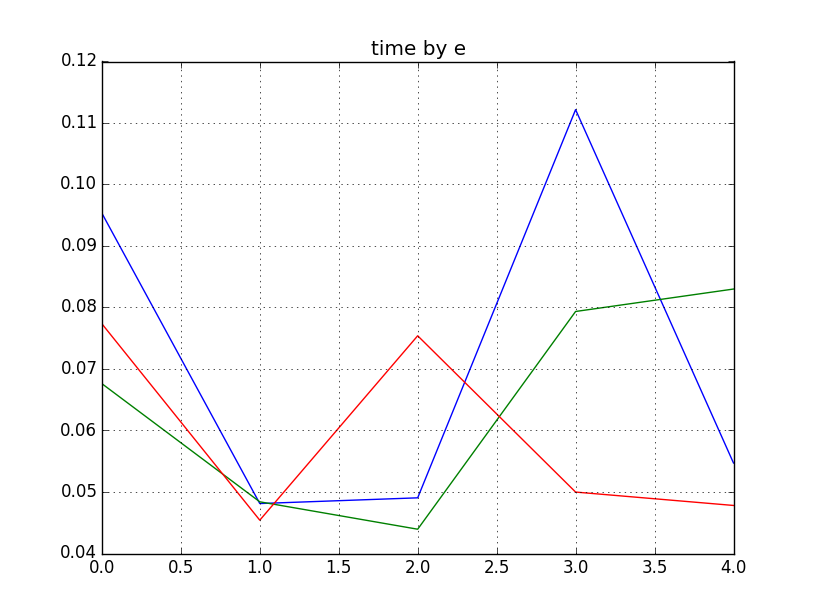
\includegraphics[width=1.1\textwidth]{img/timefor_e.png}
    \caption{ График, отображающий зависимость времени работы алгоритма от параметра e}
    \label{fig:timefor_e}
    }
\end{figure}

Как видно из \ref{fig:timefor_e}, лучшим значением параметра e является единица, т.е. оптимальной ситуацией является та, где в колонии есть один "элитный" муравей.

Для проверки значимости p, зафиксируем Q=1, $\alpha$=1, $\beta$=1 и e=1 и будем изменять e в диапазоне [0, 1] с шагом 0.1. Результаты представлены на \ref{fig:timefor_p}

\begin{figure}[ht!]
    \centering{
        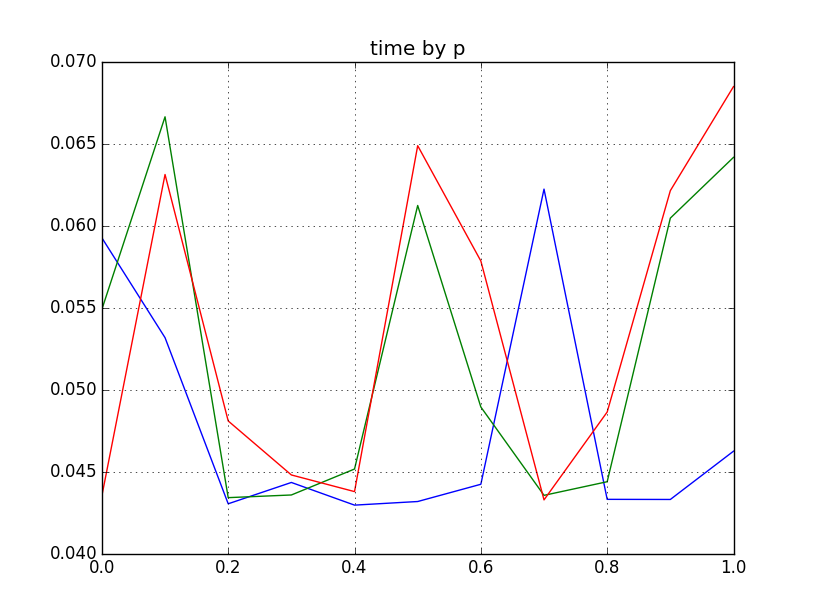
\includegraphics[width=1.1\textwidth]{img/timefor_p.png}
    \caption{ График, отображающий зависимость времени работы алгоритма от параметра p}
    \label{fig:timefor_p}
    }
\end{figure}

Как видно из \ref{fig:timefor_p} лучшим значением параметра p является 0.3.
